\documentclass[letterpaper, 10 pt, conference]{ieeeconf}  % Comment this line out if you need a4paper

%\documentclass[a4paper, 10pt, conference]{ieeeconf}      % Use this line for a4 paper

\IEEEoverridecommandlockouts                              % This command is only needed if 
                                                          % you want to use the \thanks command

\overrideIEEEmargins                                      % Needed to meet printer requirements.

% See the \addtolength command later in the file to balance the column lengths
% on the last page of the document

% The following packages can be found on http:\\www.ctan.org
\usepackage{graphicx} % for pdf, bitmapped graphics files
\graphicspath{{../}}
%\usepackage{epstopdf} % for postscript graphics files
%\usepackage{mathptmx} % assumes new font selection scheme installed
%\usepackage{times} % assumes new font selection scheme installed
%\usepackage{amsmath} % assumes amsmath package installed
%\usepackage{amssymb}  % assumes amsmath package installed

\title{\LARGE \bf
3D-PIV application for autonomous vehicles using monocular vision
}


\author{Eduardo Afonso$^{1}$ and Researcher$^{2}$% <-this % stops a space
\thanks{$^{1}$ Eduardo Afonso is coursing Control and Automation Engineering,
        Federal University of Lavras, Lavras - MG, Brazil.
        {\tt\small eduardo.afonso@engautomacao.ufla.br}}%
\thanks{$^{2}$ Researcheris with the Department of Electrical Engineering, Wright State University,
        Dayton, OH 45435, USA
        {\tt\small b.d.researcher@ieee.org}}%
}


\begin{document}


\maketitle
\thispagestyle{empty}
\pagestyle{empty}

\begin{abstract}


\end{abstract}

\section{INTRODUCTION}

Monocular vision has been demonstrating a flourishing field in autonomous vehicles.\\Several applications has presented excellent 
solutions to problems presented nowadays. Therefore, this research contributes with an innovation, using Particle Image 
Velocimetry (PIV)\cite{Bastiaans} and Pearson's Correlation Coefficient (PCC)\cite{Miranda Neto}.\\The proposal is to follow objects in scene and
stipulate its relative velocity using the both techniques cited above. These parameters are calculated in 2 and 3 dimensions, and
generated a coefficient relative to velocity of approaching and departure of objects.

Matlab is software used to validation of algorithm. PIV was the most important point of the beginning this project, considering numerous applications
\cite{Story, Xu}.\\Generally, this technique is utilized to calculate the field of velocity in fluids. 
Thus, it's possible to figure out the velocity of any objects that moves in scene. PIV was adjusted for situation to autonomous vehicles, 
using PCC and bank of dates of KITTI\cite{Geiger}.

\section{THEORETICAL FUNDAMENT}

\subsection{PEARSON CORRELATION COEFFICIENT - PCC}

PCC is used in different fields, like: statistical analyses, pattern recognition and computer vision. 
Applications include disparity measurement, object recognition and comparing two images. The followed equation
describes PCC for monochrome digital images\cite{Eugene}:

\begin{center}
$$
r_i = \frac{\sum\limits_i (x_i-x_m)(y_i-y_m)}{\sqrt{\sum\limits_i (x_i-x_m)^2} \sqrt{\sum\limits_i (y_i-y_m)^2}}
$$
\end{center}

Where $x_i$ is the intensity of the i th pixel in image 1, $y_i$ is the intensity of the i th pixel in image 2, $x_m$ is the mean intensity of
image 1, and $y_m$ is the mean intensity of image 2 \cite{Miranda Neto}.

\subsection{PARTICLE IMAGE VELOCIMETRY - PIV}

PIV is a method of determining velocity fields from images of seeded flows\cite{Bastiaans}.
This technique is used to measure velocities of part or entire image. Its results is given by 
field of vector, demonstrating direction, sense and intensity of velocity in each particles. Therefore,
it is possible to calculate the velocities of any part of image with two frames, for example.\\
PIV is powerful technique, and current researches support the vast applications \cite{Miranda Neto, Story, Xu} 
mainly involving fluids.

\section{SYSTEM DESCRIPTION}
The purpose of this algorithm is tracking objects, producing added informations about the followed target.
The algorithm developed takes inputs, such as: sequential frames and ROI(region of interesting). They are important to
define the parameters used to generate tracking of objects and more details: relative velocity and factor of approaching or departure.\\
With ROI determined, the system enters in looping to follow the target as shown in the fig. 1.

\begin{figure}[bhp]
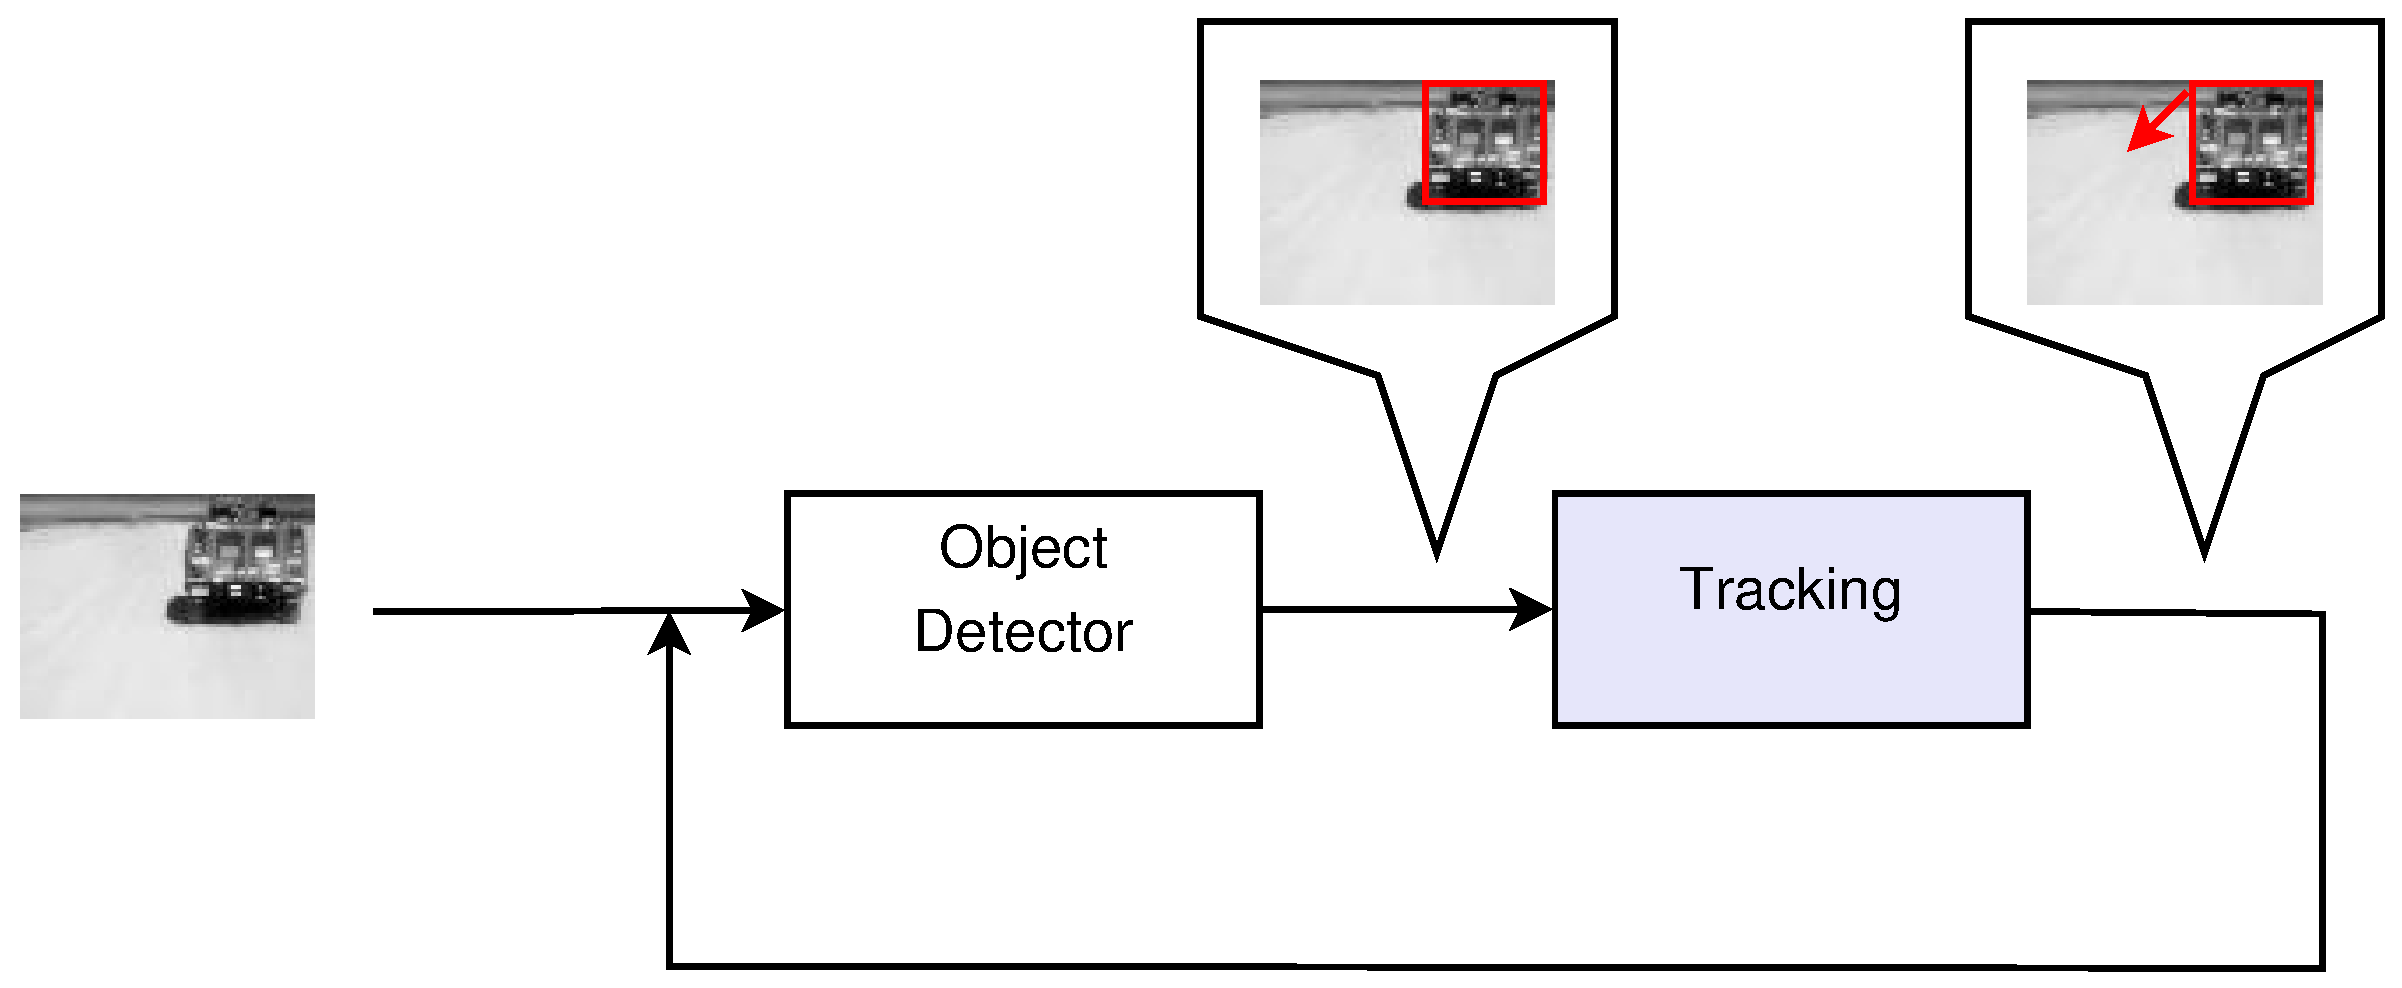
\includegraphics[width=\columnwidth]{Diagram1.eps}
\caption{Operation of algorithm in looping}
\end{figure}

In 2 dimensions, the objects are tracking and given information about its horizontal or vertical relative velocity.
When the target moves in 3 dimensions, outputs are the relative velocity and the factor of approaching or departure. So that, 
there isn't the factor in 2 dimensions, since approaching or departure don't exist in this situation.

%Diagrama1
 %A gente vai explicar o algoritmo como uma caixa fechada , que coisa entra e que coisa sai
 %e os parametros a sintonizar.
 % como usar ele quando implementado, como se fosse uma caixa preta.
 
\section{ALGORITHM DESCRIPTION}
 
%DiagramaX

\subsection{MULTI-RESOLUTION MATCH CRITERIA}
There are two method to find an object in the image in this algorithm. One is a search in axis x and y and other includes axis z.
In the first way, the parameters of ROI are used to define the window of search (WOS) and the search is made pixel by pixel for whole WOS. 
The ROI and image selected are compared and verified if they are similar in each iteration. The new place of object is found from the image 
of the highest coefficient calculated by PCC.\\
Other method to figure out the image includes axis z. In this way, the search is made in different layers and,
consequently, the WOS changes beginning of the smallest (0.8 of size of ROI) until the biggest (1.2 of size of ROI) WOS 
with increment of 0.05 in each iteration.\\

%onde estava, onde esta agora
%que tamanho tinha que tamanho tem.
\subsubsection{MULTI-PLAYER 3D APPROXIMATION}
%usa Multi-resolution match criteria e explica isso dos tamanhos

\subsubsection{FACTOR OF APPROACHING - RELATIVE VELOCITY}


\subsection{RENEW ROI CRITERIA}
%Diagrama2


% descri��o do sistemA
\section{NUMERICAL RESULTS}
%testes com diferentes parametros
% tabelas e graficos

\section{CONCLUSIONS}

PIV has presented satisfactory results. Different kinds of information that can be concluded, like: estimate collision, tracking of
objects in 2 or 3 dimensions and factor of approaching and removal. The simulations in Matlab has given promissories results: (TABLES
and GRAPHICS).

\addtolength{\textheight}{-12cm}

\section*{ACKNOWLEDGMENT}

%FAPEMIG\\
%numero de bolsa\\
%numero de projeto\\
%numero de aluno


\begin{thebibliography}{99}

\bibitem{Auoude} G.S. Auoude et al. Sampling-Based Threat Assessment Algorithms for Intersection Collisions Involving 
        Errant Drivers. IFAC Symposium on Intelligent Autonomous Vehicles, 2010.
        
	\bibitem{Bastiaans} R. J. M. Bastiaans, Cross-correlation PIV; theory, implementation and accuracy. 
        Eindhoven: Technische Universiteit Eindhoven, 2000. - EUT Report 99-W-OOl. - ISBN: 90-386-2851-X.
        
        \bibitem{Eugene} Y. K. Eugene and R.G. Johnston, The Ineffectiveness of the Correlation Coefficient for Image Comparisons.
        Technical Report LA-UR-96-2474, Los Alamos, 1996.
        
        \bibitem{Geiger} A. Geiger et al,
        Vision meets Robotics: The KITTI Dataset. International Journal of Robotics Research (IJRR), 2013.
        
        \bibitem{Jonas} T. Jonas, Real-Time Probabilistic Collision Avoidance for Autonomous Vehicles, Using Order Reductive 
        Conflict Metrics. Submitted to the Department of Aeronautics and Astronautics
	in partial fulfillment of the requirements for the degree of Doctor of Philosophy. Massachusetts Institute of Technology. June, 2003.
        
        \bibitem{Miranda Neto} A. Miranda Neto et al, Image Processing Using Pearson's Correlation Coefficient: 
        Applications on Autonomous Robotics. 
        Autonomous Robot Systems (Robotica), 2013 13th International Conference on, 2013.
	
	\bibitem{Story} A. Story et al, PIV measurements of the velocity field of a Newtonian Fluid in a stirred tank equipped 
	with the PMT type impeller.Technical Transactions - Chemistry. 2-Ch/2014.
	
	\bibitem{Woerner} K. Woerner, COLREGS-Compliant Autonomous Collision Avoidance Using Multi-Objective Optimization
	with Interval Programming. Submitted to the Department of Mechanical Engineering in partial fulfillment of the requirements for the 
	degrees of Naval Engineer and Master of Science in Mechanical Engineering. Massachusetts Institute of Technology. June, 2014.
	
	\bibitem{Xu} L. Xu, Computational fluid dynamics analysis and PIV validation of a bionic vortex flow 
	pulsatile LVAD.Technology and Health Care 23 (2015) S443?S451. DOI 10.3233/THC-150981. IOS Press, 2015.


\end{thebibliography}

\end{document}
